% =========================================================================
% BÀI 09: LUYỆN TẬP CHUNG (HÌNH PHẲNG)
% Dành cho học sinh Lớp 1 - Trực quan 100% hình vẽ TikZ sinh động
% =========================================================================

\providecommand{\VeQue}[5]{%
  \draw[line width=3.2pt, #5, line cap=round] (#1,#2) -- (#3,#4);
  \fill[red!85!black] (#1,#2) circle (2.2pt);
  \fill[red!85!black] (#3,#4) circle (2.2pt);
}

% =========================================================================
% PHẦN 1: TRẮC NGHIỆM LỰA CHỌN (12 CÂU)
% =========================================================================
\textbf{Phần 1. Trắc nghiệm lựa chọn}
\setcounterpageref{ex}{0}

% --- CÂU 1 ---
\begin{ex} %[1H2N09]
Hình nào dưới đây có 4 cạnh bằng nhau?
\begin{center}
\setlength{\tabcolsep}{8pt}
\begin{tabular}{cccc}
  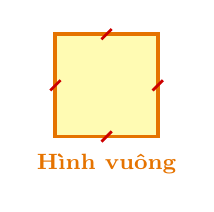
\begin{tikzpicture}[scale=0.65]
    \draw[fill=yellow!30, draw=orange!90!black, line width=1.4pt] (-1,-1) rectangle (1,1);
    \foreach \x/\y in {0/1, 1/0, 0/-1, -1/0} {
      \draw[red!80!black, line width=1pt] (\x-0.1,\y-0.1) -- (\x+0.1,\y+0.1);
    }
    \node[below=3pt, font=\footnotesize\bfseries\color{orange!90!black}] at (0,-1) {Hình vuông};
  \end{tikzpicture}
  &
  \begin{tikzpicture}[scale=0.65]
    \draw[fill=cyan!25, draw=blue!90!black, line width=1.4pt] (-1.4,-0.8) rectangle (1.4,0.8);
    \node[below=3pt, font=\footnotesize\bfseries\color{blue!90!black}] at (0,-0.8) {Hình chữ nhật};
  \end{tikzpicture}
  &
  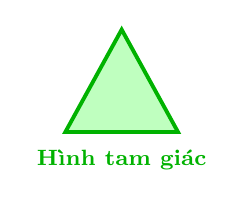
\begin{tikzpicture}[scale=0.65]
    \draw[fill=green!25, draw=green!70!black, line width=1.4pt] (-1.1,-0.9) -- (1.1,-0.9) -- (0,1.1) -- cycle;
    \node[below=3pt, font=\footnotesize\bfseries\color{green!70!black}] at (0,-0.9) {Hình tam giác};
  \end{tikzpicture}
  &
  
\begin{tikzpicture}[scale=0.65]
    \draw[fill=pink!35, draw=purple!85!black, line width=1.4pt] (0,0) circle (1.0cm);
    \node[below=3pt, font=\footnotesize\bfseries\color{purple!85!black}] at (0,-1) {Hình tròn};
  \end{tikzpicture}
\end{tabular}
\end{center}
\choice
{Hình chữ nhật}
{Hình tam giác}
{Hình tròn}
{\True Hình vuông}
\loigiai{
Hình vuông có 4 cạnh bằng nhau.\\
\textbf{Đáp án của câu hỏi là D}
}
\end{ex}

% --- CÂU 2 ---
\begin{ex} %[1H2N09]
Mặt trăng tròn ngày rằm như hình dưới đây có dạng hình gì?
\begin{center}
\begin{tikzpicture}[scale=0.85, baseline=(current bounding box.center)]
  % Nền trời đêm
  \draw[fill=blue!90!black, rounded corners=6pt, draw=blue!95!black] (-3.2,-1.05) rectangle (3.2,1.05);
  % Ngôi sao nhỏ
  \foreach \sx/\sy in {-2.5/0.55, -1.8/-0.5, -2.2/0.1, 1.8/0.65, 2.4/-0.4, 2.0/0.2} {
    \fill[yellow!90!white] (\sx,\sy) circle (0.05cm);
  }
  % Trăng rằm vàng rực rỡ
  \draw[fill=yellow!90!orange, draw=orange!90!black, line width=1.5pt] (0,0) circle (0.85cm);
  % Khuôn mặt trăng cười dễ thương
  \fill[brown!70!black] (-0.28,0.18) circle (0.07cm);
  \fill[brown!70!black] (0.28,0.18) circle (0.07cm);
  \draw[line width=1.2pt, brown!80!black] (-0.2,-0.12) arc (190:350:0.2cm);
  \fill[pink!70!red, opacity=0.7] (-0.45,0.05) circle (0.09cm);
  \fill[pink!70!red, opacity=0.7] (0.45,0.05) circle (0.09cm);
  \node[font=\footnotesize\bfseries\color{white}] at (0,-0.75) {Mặt trăng ngày rằm};
\end{tikzpicture}
\end{center}
\choice
{\True Hình tròn}
{Hình vuông}
{Hình tam giác}
{Hình chữ nhật}
\loigiai{
Mặt trăng rằm có dạng \textbf{hình tròn}.\\
\textbf{Đáp án của câu hỏi là A}
}
\end{ex}

% --- CÂU 3 ---
\begin{ex} %[1H2H09]
Khung cửa ra vào lớp học có dạng hình gì?
\begin{center}
\begin{tikzpicture}[scale=0.8, baseline=(current bounding box.center)]
  % Khung cửa ngoài
  \draw[fill=brown!40, draw=brown!85!black, line width=1.4pt] (-1.0,-1.25) rectangle (1.0,1.25);
  % Cánh cửa trong
  \draw[fill=orange!25, draw=brown!80!black, line width=1.1pt] (-0.85,-1.1) rectangle (0.85,1.1);
  % Ô kính nhỏ trên cửa
  \draw[fill=cyan!30, draw=blue!70!black, line width=1pt] (-0.6,0.25) rectangle (0.6,0.9);
  \draw[blue!70!black, line width=0.8pt] (0,0.25) -- (0,0.9);
  \draw[blue!70!black, line width=0.8pt] (-0.6,0.575) -- (0.6,0.575);
  % Tay nắm cửa tròn
  \fill[yellow!80!black] (0.65,-0.1) circle (0.08cm);
  \node[below=2pt, font=\small\bfseries\color{brown!85!black}] at (0,-1.25) {Khung cửa ra vào};
\end{tikzpicture}
\end{center}
\choice
{\True Hình chữ nhật}
{Hình tam giác}
{Hình tròn}
{Hình vuông}
\loigiai{
Khung cửa ra vào có dạng \textbf{hình chữ nhật}.\\
\textbf{Đáp án của câu hỏi là A}
}
\end{ex}

% --- CÂU 4 ---
\begin{ex} %[1H2H09]
Đếm số đỉnh (chấm tròn đỏ) của hình tam giác dưới đây:
\begin{center}
\begin{tikzpicture}[scale=0.85, baseline=(current bounding box.center)]
  \draw[fill=green!25, draw=green!70!black, line width=1.4pt] (-1.4,-0.7) -- (1.4,-0.7) -- (0,1.2) -- cycle;
  % 3 đỉnh với chấm đỏ và nhãn
  \fill[red!85!black] (-1.4,-0.7) circle (0.11cm);
  \fill[red!85!black] (1.4,-0.7) circle (0.11cm);
  \fill[red!85!black] (0,1.2) circle (0.11cm);
  \node[above=2pt, font=\small\bfseries\color{red!85!black}] at (0,1.2) {Đỉnh 1};
  \node[left=3pt, font=\small\bfseries\color{red!85!black}] at (-1.4,-0.7) {Đỉnh 2};
  \node[right=3pt, font=\small\bfseries\color{red!85!black}] at (1.4,-0.7) {Đỉnh 3};
\end{tikzpicture}
\end{center}
\choice
{$2$ đỉnh}
{$4$ đỉnh}
{$5$ đỉnh}
{\True $3$ đỉnh}
\loigiai{
Hình tam giác có \textbf{3 đỉnh}.\\
\textbf{Đáp án của câu hỏi là D}
}
\end{ex}

\newpage
% --- CÂU 5 ---
\begin{ex} %[1H2H09]
Hình chữ nhật dưới đây có bao nhiêu cạnh?
\begin{center}
\begin{tikzpicture}[scale=0.85, baseline=(current bounding box.center)]
  \draw[fill=cyan!20, draw=blue!90!black, line width=1.4pt] (-1.9,-0.8) rectangle (1.9,0.8);
  \node[above=2pt, font=\small\bfseries\color{blue!90!black}] at (0,0.8) {Cạnh 1};
  \node[right=3pt, font=\small\bfseries\color{blue!90!black}] at (1.9,0) {Cạnh 2};
  \node[below=2pt, font=\small\bfseries\color{blue!90!black}] at (0,-0.8) {Cạnh 3};
  \node[left=3pt, font=\small\bfseries\color{blue!90!black}] at (-1.9,0) {Cạnh 4};
\end{tikzpicture}
\end{center}
\choice
{$3$ cạnh}
{$5$ cạnh}
{\True $4$ cạnh}
{$6$ cạnh}
\loigiai{
Hình chữ nhật có \textbf{4 cạnh}.\\
\textbf{Đáp án của câu hỏi là C}
}
\end{ex}

% --- CÂU 6 ---
\begin{ex} %[1H2H09]
Dùng 6 que tính xếp được 2 hình gì như hình vẽ dưới đây?
\begin{center}
\setlength{\tabcolsep}{15pt}
\begin{tabular}{cc}
  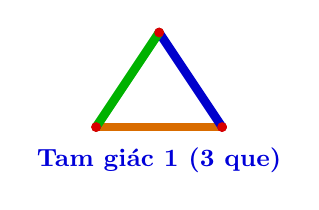
\begin{tikzpicture}[scale=0.8]
    \VeQue{-1.0}{-0.6}{1.0}{-0.6}{orange!85!black}
    \VeQue{1.0}{-0.6}{0}{0.9}{blue!80!black}
    \VeQue{0}{0.9}{-1.0}{-0.6}{green!70!black}
    \node[below=4pt, font=\small\bfseries\color{blue!85!black}] at (0,-0.6) {Tam giác 1 (3 que)};
  \end{tikzpicture}
  &
  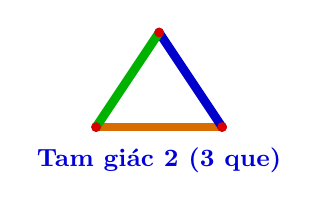
\begin{tikzpicture}[scale=0.8]
    \VeQue{-1.0}{-0.6}{1.0}{-0.6}{orange!85!black}
    \VeQue{1.0}{-0.6}{0}{0.9}{blue!80!black}
    \VeQue{0}{0.9}{-1.0}{-0.6}{green!70!black}
    \node[below=4pt, font=\small\bfseries\color{blue!85!black}] at (0,-0.6) {Tam giác 2 (3 que)};
  \end{tikzpicture}
\end{tabular}
\end{center}
\choice
{\True 2 hình tam giác}
{2 hình vuông}
{2 hình chữ nhật}
{2 hình tròn}
\loigiai{
Mỗi hình tam giác cần 3 que tính. 6 que tính xếp được \textbf{2 hình tam giác}.\\
\textbf{Đáp án của câu hỏi là A}
}
\end{ex}

% --- CÂU 7 ---
\begin{ex} %[1H2V09]
Trong 4 hình dưới đây, hình nào KHÔNG có góc hay đỉnh nào?
\begin{center}
\setlength{\tabcolsep}{8pt}
\begin{tabular}{cccc}
  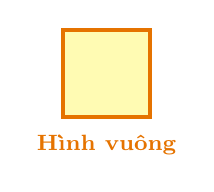
\begin{tikzpicture}[scale=0.65]
    \draw[fill=yellow!30, draw=orange!90!black, line width=1.4pt] (-0.85,-0.85) rectangle (0.85,0.85);
    \node[below=3pt, font=\footnotesize\bfseries\color{orange!90!black}] at (0,-0.85) {Hình vuông};
  \end{tikzpicture}
  &
  
\begin{tikzpicture}[scale=0.65]
    \draw[fill=pink!40, draw=purple!85!black, line width=1.4pt] (0,0) circle (0.9cm);
    \node[below=3pt, font=\footnotesize\bfseries\color{purple!85!black}] at (0,-0.9) {Hình tròn};
  \end{tikzpicture}
  &
  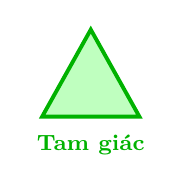
\begin{tikzpicture}[scale=0.65]
    \draw[fill=green!25, draw=green!70!black, line width=1.4pt] (-0.95,-0.75) -- (0.95,-0.75) -- (0,0.95) -- cycle;
    \node[below=3pt, font=\footnotesize\bfseries\color{green!70!black}] at (0,-0.75) {Tam giác};
  \end{tikzpicture}
  &
  \begin{tikzpicture}[scale=0.65]
    \draw[fill=cyan!25, draw=blue!90!black, line width=1.4pt] (-1.2,-0.7) rectangle (1.2,0.7);
    \node[below=3pt, font=\footnotesize\bfseries\color{blue!90!black}] at (0,-0.7) {Chữ nhật};
  \end{tikzpicture}
\end{tabular}
\end{center}
\choice
{Hình tam giác}
{Hình vuông}
{\True Hình tròn}
{Hình chữ nhật}
\loigiai{
Hình tròn là đường cong tròn khép kín, \textbf{không có góc hay đỉnh}.\\
\textbf{Đáp án của câu hỏi là C}
}
\end{ex}

% --- CÂU 8 ---
\begin{ex} %[1H2V09]
Quan sát hình vẽ: có 3 hình tam giác và 4 hình vuông. Tổng số hình là bao nhiêu?
\begin{center}
\setlength{\tabcolsep}{15pt}
\begin{tabular}{cc}
  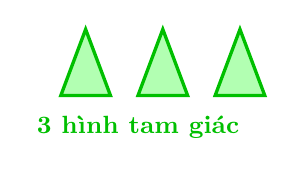
\begin{tikzpicture}[scale=0.7]
    \foreach \i in {0,1,2} {
      \draw[fill=green!30, draw=green!75!black, line width=1.2pt] (\i*1.4-1.4, -0.55) -- (\i*1.4-0.5, -0.55) -- (\i*1.4-0.95, 0.65) -- cycle;
    }
    \node[below=4pt, font=\small\bfseries\color{green!75!black}] at (0,-0.55) {3 hình tam giác};
  \end{tikzpicture}
  &
  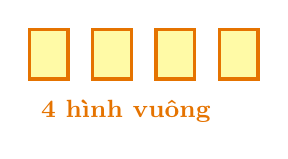
\begin{tikzpicture}[scale=0.7]
    \foreach \i in {0,1,2,3} {
      \draw[fill=yellow!35, draw=orange!90!black, line width=1.2pt] (\i*1.15-1.75, -0.45) rectangle (\i*1.15-1.05, 0.45);
    }
    \node[below=4pt, font=\small\bfseries\color{orange!90!black}] at (0,-0.45) {4 hình vuông};
  \end{tikzpicture}
\end{tabular}
\end{center}
\choice
{$6$ hình}
{\True $7$ hình}
{$8$ hình}
{$9$ hình}
\loigiai{
$3 + 4 = \textbf{7 hình}$.\\
\textbf{Đáp án của câu hỏi là B}
}
\end{ex}

\newpage
% --- CÂU 9 ---
\begin{ex} %[1H2V09]
Cần bao nhiêu que tính để xếp được 1 hình vuông và 1 hình tam giác riêng biệt như hình dưới?
\begin{center}
\setlength{\tabcolsep}{18pt}
\begin{tabular}{cc}
  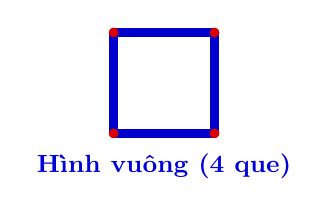
\begin{tikzpicture}[scale=0.8]
    \VeQue{-0.8}{-0.8}{0.8}{-0.8}{blue!80!black}
    \VeQue{0.8}{-0.8}{0.8}{0.8}{blue!80!black}
    \VeQue{0.8}{0.8}{-0.8}{0.8}{blue!80!black}
    \VeQue{-0.8}{0.8}{-0.8}{-0.8}{blue!80!black}
    \node[below=4pt, font=\small\bfseries\color{blue!85!black}] at (0,-0.8) {Hình vuông (4 que)};
  \end{tikzpicture}
  &
  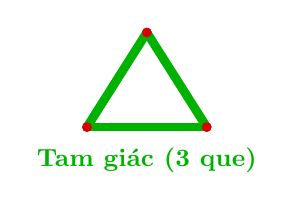
\begin{tikzpicture}[scale=0.8]
    \VeQue{-0.95}{-0.65}{0.95}{-0.65}{green!70!black}
    \VeQue{0.95}{-0.65}{0}{0.85}{green!70!black}
    \VeQue{0}{0.85}{-0.95}{-0.65}{green!70!black}
    \node[below=4pt, font=\small\bfseries\color{green!70!black}] at (0,-0.65) {Tam giác (3 que)};
  \end{tikzpicture}
\end{tabular}
\end{center}
\choice
{$6$ que}
{\True $7$ que}
{$8$ que}
{$9$ que}
\loigiai{
Số que tính cần dùng là: $4 + 3 = \textbf{7 que tính}$.\\
\textbf{Đáp án của câu hỏi là B}
}
\end{ex}

% --- CÂU 10 ---
\begin{ex} %[1H2V09]
Ghép 2 hình tam giác bằng nhau như hình dưới đây, ta được hình gì?
\begin{center}
\begin{tikzpicture}[scale=0.85, baseline=(current bounding box.center)]
  % Tam giác 1
  \draw[fill=yellow!40, draw=orange!90!black, line width=1.4pt] (-1.1,-1.1) -- (1.1,-1.1) -- (-1.1,1.1) -- cycle;
  \node[font=\small\bfseries\color{orange!90!black}] at (-0.45,-0.45) {1};
  % Tam giác 2
  \draw[fill=cyan!35, draw=blue!90!black, line width=1.4pt] (1.1,-1.1) -- (1.1,1.1) -- (-1.1,1.1) -- cycle;
  \node[font=\small\bfseries\color{blue!90!black}] at (0.45,0.45) {2};
  % Đường chéo ghép
  \draw[red!80!black, dashed, line width=1.4pt] (-1.1,1.1) -- (1.1,-1.1);
  \node[below=4pt, font=\small\bfseries\color{purple!80!black}] at (0,-1.1) {2 hình tam giác ghép lại};
\end{tikzpicture}
\end{center}
\choice
{Hình tròn}
{Hình có 5 cạnh}
{Khối lập phương}
{\True Hình vuông}
\loigiai{
Ghép 2 tam giác vuông cân bằng nhau ta được một \textbf{hình vuông}.\\
\textbf{Đáp án của câu hỏi là D}
}
\end{ex}

% --- CÂU 11 ---
\begin{ex} %[1H2V09]
Biển báo giao thông cấm đi ngược chiều dưới đây có dạng hình gì?
\begin{center}
\begin{tikzpicture}[scale=0.85, baseline=(current bounding box.center)]
  % Biển tròn đỏ viền trắng
  \draw[fill=red!90!black, draw=red!95!black, line width=1.2pt] (0,0) circle (1.05cm);
  \draw[white, line width=1.5pt] (0,0) circle (0.97cm);
  % Vạch trắng ngang ở giữa
  \draw[fill=white, draw=none, rounded corners=1.5pt] (-0.7,-0.17) rectangle (0.7,0.17);
  % Cột biển báo
  \draw[fill=gray!60, draw=gray!80!black, line width=1pt] (-0.08,-1.05) rectangle (0.08,-1.65);
  \node[below=2pt, font=\small\bfseries\color{red!90!black}] at (0,-1.65) {Biển báo giao thông};
\end{tikzpicture}
\end{center}
\choice
{Hình vuông}
{Hình tam giác}
{\True Hình tròn}
{Hình chữ nhật}
\loigiai{
Biển báo cấm đi ngược chiều có dạng \textbf{hình tròn}.\\
\textbf{Đáp án của câu hỏi là C}
}
\end{ex}

% --- CÂU 12 ---
\begin{ex} %[1H2C09]
Bé vẽ con lật đật gồm 1 hình tròn nhỏ làm đầu và 1 hình tròn lớn làm thân như hình vẽ. Hỏi hình con lật đật gồm mấy hình tròn?
\begin{center}
\begin{tikzpicture}[scale=0.8, baseline=(current bounding box.center)]
  % Thân hình tròn lớn
  \draw[fill=red!75!orange, draw=red!90!black, line width=1.4pt] (0,-0.4) circle (0.85cm);
  % Họa tiết bụng lật đật
  \draw[fill=yellow!90!white, draw=orange!80!black, line width=1pt] (0,-0.4) circle (0.45cm);
  \fill[red!80!black] (0,-0.3) circle (0.07cm);
  \fill[red!80!black] (0,-0.55) circle (0.07cm);
  % 2 tay tròn nhỏ
  \draw[fill=red!75!orange, draw=red!90!black, line width=1.2pt] (-0.95,-0.3) circle (0.2cm);
  \draw[fill=red!75!orange, draw=red!90!black, line width=1.2pt] (0.95,-0.3) circle (0.2cm);
  % Đầu hình tròn nhỏ
  \draw[fill=pink!35, draw=orange!90!black, line width=1.4pt] (0,0.85) circle (0.55cm);
  % Mắt mũi miệng
  \fill[black] (-0.18,0.95) circle (0.05cm);
  \fill[black] (0.18,0.95) circle (0.05cm);
  \draw[line width=1pt, red!85!black] (-0.12,0.75) arc (190:350:0.12cm);
  \fill[pink!80!red, opacity=0.7] (-0.32,0.83) circle (0.07cm);
  \fill[pink!80!red, opacity=0.7] (0.32,0.83) circle (0.07cm);
  % Chỏm mũ
  \draw[fill=red!80!black, draw=none] (-0.2,1.35) -- (0,1.6) -- (0.2,1.35) -- cycle;
  % Nhãn
  \node[font=\footnotesize\bfseries\color{blue!90!black}] at (1.4,0.85) {1. Đầu};
  \draw[->, >=stealth, line width=0.8pt, blue!90!black] (0.95,0.85) -- (0.6,0.85);
  \node[font=\footnotesize\bfseries\color{red!90!black}] at (1.6,-0.4) {2. Thân};
  \draw[->, >=stealth, line width=0.8pt, red!90!black] (1.1,-0.4) -- (0.9, -0.4);
\end{tikzpicture}
\end{center}
\choice
{$1$ hình}
{\True $2$ hình}
{$3$ hình}
{$4$ hình}
\loigiai{
Con lật đật gồm \textbf{2 hình tròn}: 1 hình tròn nhỏ làm đầu và 1 hình tròn lớn làm thân.\\
\textbf{Đáp án của câu hỏi là B}
}
\end{ex}

\newpage
% =========================================================================
% PHẦN 2: TRẮC NGHIỆM ĐÚNG SAI (2 CÂU)
% =========================================================================
\textbf{Phần 2. Trắc nghiệm đúng sai (Quan sát hình vẽ và xét tính đúng/sai)}
\setcounterpageref{ex}{0}

% --- CÂU 13 ---
\begin{ex} %[1H2H09]
Quan sát các hình phẳng dưới đây:
\begin{center}
\setlength{\tabcolsep}{8pt}
\begin{tabular}{ccc}
  \begin{tikzpicture}[scale=0.7]
    \draw[fill=green!25, draw=green!70!black, line width=1.4pt] (-1.0,-0.65) -- (1.0,-0.65) -- (0,1.0) -- cycle;
    \fill[red!85!black] (-1.0,-0.65) circle (0.1cm);
    \fill[red!85!black] (1.0,-0.65) circle (0.1cm);
    \fill[red!85!black] (0,1.0) circle (0.1cm);
    \node[below=3pt, font=\footnotesize\bfseries\color{green!70!black}] at (0,-0.65) {Tam giác: 3 cạnh, 3 đỉnh};
  \end{tikzpicture}
  &
  \begin{tikzpicture}[scale=0.7]
    \draw[fill=cyan!25, draw=blue!90!black, line width=1.4pt] (-1.2,-0.65) rectangle (1.2,0.65);
    \node[below=3pt, font=\footnotesize\bfseries\color{blue!90!black}] at (0,-0.65) {Chữ nhật: 4 cạnh};
  \end{tikzpicture}
  &
  \begin{tikzpicture}[scale=0.7]
    \draw[fill=pink!35, draw=purple!85!black, line width=1.4pt] (0,0) circle (0.8cm);
    \node[below=3pt, font=\footnotesize\bfseries\color{purple!85!black}] at (0,-0.8) {Tròn: không có đỉnh};
  \end{tikzpicture}
\end{tabular}
\end{center}
Xét tính đúng sai của các câu sau:
\choiceTF
{\True Hình tam giác có 3 cạnh.}
{\True Hình chữ nhật có 4 cạnh.}
{Hình tròn có 4 đỉnh.}
{\True Hình tròn là đường cong tròn khép kín, không có đỉnh.}
\loigiai{
\begin{itemize}
    \item a) \textbf{Đúng}: Tam giác có 3 cạnh.
    \item b) \textbf{Đúng}: Hình chữ nhật có 4 cạnh.
    \item c) \textbf{Sai}: Hình tròn không có đỉnh nào.
    \item d) \textbf{Đúng}: Hình tròn là đường cong khép kín, không có góc hay đỉnh.
\end{itemize}
}
\end{ex}

% --- CÂU 14 ---
\begin{ex} %[1H2V09]
Trong bộ đồ dùng học tập của bạn Mai có các hình như sau:
\begin{center}
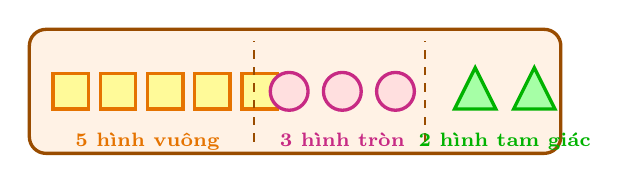
\begin{tikzpicture}[scale=0.75, baseline=(current bounding box.center)]
  % Khay đựng hình
  \draw[fill=orange!10, draw=orange!60!black, line width=1.2pt, rounded corners=6pt] (-4.5,-1.05) rectangle (4.5,1.05);
  % 5 hình vuông vàng
  \foreach \i in {0,1,2,3,4} {
    \draw[fill=yellow!40, draw=orange!90!black, line width=1.2pt] (\i*0.8-4.1, -0.3) rectangle (\i*0.8-3.5, 0.3);
  }
  \node[below=2pt, font=\scriptsize\bfseries\color{orange!90!black}] at (-2.5,-0.45) {5 hình vuông};
  % Vách ngăn
  \draw[dashed, line width=0.8pt, orange!60!black] (-0.7,-0.85) -- (-0.7,0.85);
  % 3 hình tròn hồng
  \foreach \i in {0,1,2} {
    \draw[fill=pink!50, draw=magenta!80!black, line width=1.2pt] (\i*0.9-0.1, 0) circle (0.32cm);
  }
  \node[below=2pt, font=\scriptsize\bfseries\color{magenta!80!black}] at (0.8,-0.45) {3 hình tròn};
  % Vách ngăn
  \draw[dashed, line width=0.8pt, orange!60!black] (2.2,-0.85) -- (2.2,0.85);
  % 2 hình tam giác xanh
  \foreach \i in {0,1} {
    \draw[fill=green!35, draw=green!70!black, line width=1.2pt] (\i*1.0+2.7, -0.3) -- (\i*1.0+3.4, -0.3) -- (\i*1.0+3.05, 0.4) -- cycle;
  }
  \node[below=2pt, font=\scriptsize\bfseries\color{green!70!black}] at (3.55,-0.45) {2 hình tam giác};
\end{tikzpicture}
\end{center}
Xét tính đúng sai của các câu sau:
\choiceTF
{\True Số hình vuông nhiều nhất (5 hình).}
{\True Số hình tam giác ít nhất (2 hình).}
{Tổng số hình trong bộ đồ dùng là 12 hình.}
{\True Tổng số hình là $5 + 3 + 2 = 10$ hình.}
\loigiai{
\begin{itemize}
    \item a) \textbf{Đúng}: 5 hình vuông > 3 hình tròn > 2 tam giác. Hình vuông nhiều nhất.
    \item b) \textbf{Đúng}: 2 hình tam giác là ít nhất.
    \item c) \textbf{Sai}: Tổng số hình là 10 hình, không phải 12.
    \item d) \textbf{Đúng}: $5 + 3 + 2 = 10$ hình.
\end{itemize}
}
\end{ex}

% =========================================================================
% PHẦN 3: TRẢ LỜI NGẮN (ĐIỀN SỐ THÍCH HỢP)
% =========================================================================
\textbf{Phần 3. Trả lời ngắn (Quan sát hình vẽ và điền số thích hợp)}
\setcounterpageref{ex}{0}

% --- CÂU 15 ---
\begin{ex} %[1H2H09]
Quan sát hình dưới đây và cho biết hình chữ nhật có bao nhiêu cạnh?
\begin{center}
\begin{tikzpicture}[scale=0.8, baseline=(current bounding box.center)]
  \draw[fill=cyan!25, draw=blue!90!black, line width=1.4pt] (-1.8,-0.75) rectangle (1.8,0.75);
  \node[above=2pt, font=\small\bfseries\color{blue!90!black}] at (0,0.75) {Cạnh 1};
  \node[right=3pt, font=\small\bfseries\color{blue!90!black}] at (1.8,0) {Cạnh 2};
  \node[below=2pt, font=\small\bfseries\color{blue!90!black}] at (0,-0.75) {Cạnh 3};
  \node[left=3pt, font=\small\bfseries\color{blue!90!black}] at (-1.8,0) {Cạnh 4};
\end{tikzpicture}
\end{center}
\shortans{4}
\loigiai{
\textbf{Đáp số:} $4$\\
Hình chữ nhật có $4$ cạnh.
}
\end{ex}

% --- CÂU 16 ---
\begin{ex} %[1H2H09]
Quan sát các chấm tròn đỏ trên hình và cho biết hình tam giác có bao nhiêu đỉnh?
\begin{center}
\begin{tikzpicture}[scale=0.8, baseline=(current bounding box.center)]
  \draw[fill=green!25, draw=green!70!black, line width=1.4pt] (-1.3,-0.65) -- (1.3,-0.65) -- (0,1.1) -- cycle;
  \fill[red!85!black] (0,1.1) circle (0.11cm);
  \node[above=2pt, font=\small\bfseries\color{red!85!black}] at (0,1.1) {Đỉnh 1};
  \fill[red!85!black] (-1.3,-0.65) circle (0.11cm);
  \node[left=2pt, font=\small\bfseries\color{red!85!black}] at (-1.3,-0.65) {Đỉnh 2};
  \fill[red!85!black] (1.3,-0.65) circle (0.11cm);
  \node[right=2pt, font=\small\bfseries\color{red!85!black}] at (1.3,-0.65) {Đỉnh 3};
\end{tikzpicture}
\end{center}
\shortans{3}
\loigiai{
\textbf{Đáp số:} $3$\\
Hình tam giác có $3$ đỉnh.
}
\end{ex}

\newpage
% --- CÂU 17 ---
\begin{ex} %[1H2V09]
Quan sát hình vẽ: cần bao nhiêu que tính để xếp được 2 hình tam giác riêng biệt?
\begin{center}
\setlength{\tabcolsep}{15pt}
\begin{tabular}{cc}
  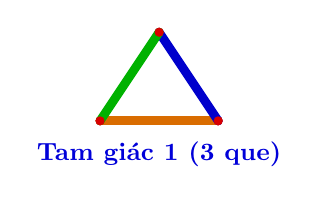
\begin{tikzpicture}[scale=0.75]
    \VeQue{-1.0}{-0.6}{1.0}{-0.6}{orange!85!black}
    \VeQue{1.0}{-0.6}{0}{0.9}{blue!80!black}
    \VeQue{0}{0.9}{-1.0}{-0.6}{green!70!black}
    \node[below=4pt, font=\small\bfseries\color{blue!85!black}] at (0,-0.6) {Tam giác 1 (3 que)};
  \end{tikzpicture}
  &
  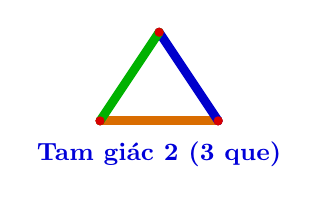
\begin{tikzpicture}[scale=0.75]
    \VeQue{-1.0}{-0.6}{1.0}{-0.6}{orange!85!black}
    \VeQue{1.0}{-0.6}{0}{0.9}{blue!80!black}
    \VeQue{0}{0.9}{-1.0}{-0.6}{green!70!black}
    \node[below=4pt, font=\small\bfseries\color{blue!85!black}] at (0,-0.6) {Tam giác 2 (3 que)};
  \end{tikzpicture}
\end{tabular}
\end{center}
\shortans{6}
\loigiai{
\textbf{Đáp số:} $6$\\
$3 \times 2 = 6$ que tính.
}
\end{ex}

% --- CÂU 18 ---
\begin{ex} %[1H2V09]
Quan sát hình vẽ: cần bao nhiêu que tính để xếp được 2 hình vuông riêng biệt?
\begin{center}
\setlength{\tabcolsep}{15pt}
\begin{tabular}{cc}
  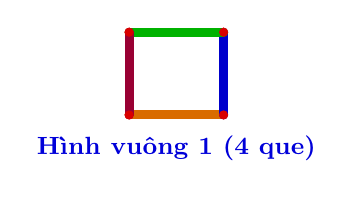
\begin{tikzpicture}[scale=0.75]
    \VeQue{-0.8}{-0.7}{0.8}{-0.7}{orange!85!black}
    \VeQue{0.8}{-0.7}{0.8}{0.7}{blue!80!black}
    \VeQue{0.8}{0.7}{-0.8}{0.7}{green!70!black}
    \VeQue{-0.8}{0.7}{-0.8}{-0.7}{purple!80!black}
    \node[below=4pt, font=\small\bfseries\color{blue!85!black}] at (0,-0.7) {Hình vuông 1 (4 que)};
  \end{tikzpicture}
  &
  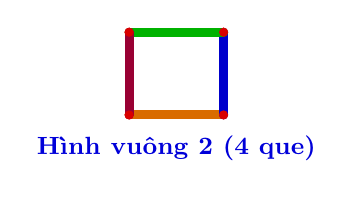
\begin{tikzpicture}[scale=0.75]
    \VeQue{-0.8}{-0.7}{0.8}{-0.7}{orange!85!black}
    \VeQue{0.8}{-0.7}{0.8}{0.7}{blue!80!black}
    \VeQue{0.8}{0.7}{-0.8}{0.7}{green!70!black}
    \VeQue{-0.8}{0.7}{-0.8}{-0.7}{purple!80!black}
    \node[below=4pt, font=\small\bfseries\color{blue!85!black}] at (0,-0.7) {Hình vuông 2 (4 que)};
  \end{tikzpicture}
\end{tabular}
\end{center}
\shortans{8}
\loigiai{
\textbf{Đáp số:} $8$\\
$4 \times 2 = 8$ que tính.
}
\end{ex}

% --- CÂU 19 ---
\begin{ex} %[1H2V09]
Quan sát hình vẽ dưới đây. Có tất cả bao nhiêu hình phẳng?
\begin{center}
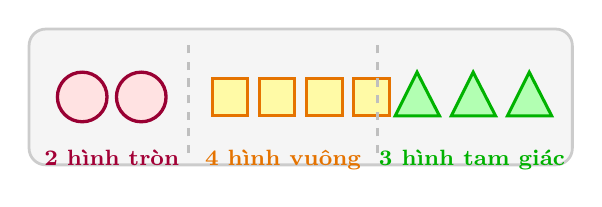
\begin{tikzpicture}[scale=0.75, baseline=(current bounding box.center)]
  % Khung nền
  \draw[fill=gray!8, draw=gray!40, line width=1pt, rounded corners=6pt] (-4.6,-1.15) rectangle (4.6,1.15);
  % 2 hình tròn
  \draw[fill=pink!45, draw=purple!80!black, line width=1.2pt] (-3.7,0) circle (0.42cm);
  \draw[fill=pink!45, draw=purple!80!black, line width=1.2pt] (-2.7,0) circle (0.42cm);
  \node[below=4pt, font=\footnotesize\bfseries\color{purple!85!black}] at (-3.2,-0.55) {2 hình tròn};
  % Vách ngăn 1
  \draw[dashed, line width=0.8pt, gray!50] (-1.9,-0.95) -- (-1.9,0.95);
  % 4 hình vuông
  \foreach \i in {0,1,2,3} {
    \draw[fill=yellow!35, draw=orange!90!black, line width=1.1pt] (\i*0.8-1.5, -0.32) rectangle (\i*0.8-0.9, 0.32);
  }
  \node[below=4pt, font=\footnotesize\bfseries\color{orange!90!black}] at (-0.3,-0.55) {4 hình vuông};
  % Vách ngăn 2
  \draw[dashed, line width=0.8pt, gray!50] (1.3,-0.95) -- (1.3,0.95);
  % 3 hình tam giác
  \foreach \i in {0,1,2} {
    \draw[fill=green!30, draw=green!70!black, line width=1.1pt] (\i*0.95+1.6, -0.32) -- (\i*0.95+2.35, -0.32) -- (\i*0.95+1.97, 0.42) -- cycle;
  }
  \node[below=4pt, font=\footnotesize\bfseries\color{green!70!black}] at (2.9,-0.55) {3 hình tam giác};
\end{tikzpicture}
\end{center}
\shortans{9}
\loigiai{
\textbf{Đáp số:} $9$\\
Tổng số hình là: $2 + 4 + 3 = 9$ hình.
}
\end{ex}

% --- CÂU 20 ---
\begin{ex} %[1H2C09]
Có 10 que tính, Nam xếp được 2 hình tam giác như hình vẽ. Hỏi Nam còn thừa mấy que tính?
\begin{center}
\setlength{\tabcolsep}{15pt}
\begin{tabular}{cc}
  \begin{tikzpicture}[scale=0.75]
    % Tam giác 1
    \VeQue{-2.2}{-0.6}{-0.2}{-0.6}{orange!85!black}
    \VeQue{-0.2}{-0.6}{-1.2}{0.9}{blue!80!black}
    \VeQue{-1.2}{0.9}{-2.2}{-0.6}{green!70!black}
    % Tam giác 2
    \VeQue{0.4}{-0.6}{2.4}{-0.6}{orange!85!black}
    \VeQue{2.4}{-0.6}{1.4}{0.9}{blue!80!black}
    \VeQue{1.4}{0.9}{0.4}{-0.6}{green!70!black}
    \node[below=4pt, font=\small\bfseries\color{blue!85!black}] at (0.1,-0.6) {Đã xếp: 2 tam giác (6 que)};
  \end{tikzpicture}
  &
  \begin{tikzpicture}[scale=0.75]
    \foreach \i in {0,1,2,3} {
      \VeQue{\i*0.6-0.9}{-0.6}{\i*0.6-0.9}{0.7}{orange!85!black}
    }
    \node[below=4pt, font=\small\bfseries\color{orange!90!black}] at (0,-0.6) {Còn thừa: ? que};
  \end{tikzpicture}
\end{tabular}
\end{center}
\shortans{4}
\loigiai{
\textbf{Đáp số:} $4$\\
Đã dùng: $3 \times 2 = 6$ que tính. Còn thừa: $10 - 6 = 4$ que tính.
}
\end{ex}
